\chapter{相关工作}

本章将深入分析相关技术领域的理论基础和发展现状,为后续系统设计提供理论支撑。基于第一章提出的研究问题,本章将从战术数据链技术、微服务架构和语义互操作三个核心方向进行详细阐述,系统梳理相关技术的理论基础、发展历程、技术特点和应用实践,为构建基于MIL-STD-6016标准的战术数据链信息标准数据库系统奠定坚实的理论基础。

\section{战术数据链(Tactical Data Link)}
战术数据链(Tactical Data Link, TDL)是实现作战平台、传感器与指挥控制中心之间实时数据传输与信息共享的核心通信方式\cite{AFMAN_13_116_Vol1_2020,EverythingRF_Link16_Band}。  
自20世纪70年代起,随着 {JTIDS} 与 {Link16} 的逐步形成,战术数据链体系不断发展,已成为现代联合作战的重要基础设施\cite{DLS_MIDS_JTRS_2021,BAE_Link16_Terminals_2025}。

战术数据链的研究早已有之,由于当时美军要求多种平台之间在电磁环境中相互协同配合进行作战,而当时的战术数据链多为模拟式信号传输,如Link4A、Link11等,虽能满足当时的需求,但具有一定的脆弱性、传输率低、网络空间小,但随着数字化通信的进步,以Link16为代表的数字化战术数据链应运而生,战术数据链的发展时代也从此开始。

现代的战术数据链具备实时性、可靠性、安全性、互操作性。实时性就是毫秒级时间内传输和处理关键信息,对于时间要求高的作战任务来说非常重要。可靠性是在电磁环境恶劣、战场环境复杂的条件下保证稳定可靠的传输。安全性是在加密算法、反干扰等方面不使通信信息被对方获取和干扰。互操作性是不同国家、不同军种间能够相互分享信息并协同作战,是现代化作战的基本要求。

在技术架构方面,战术数据链在物理层、数据链路层、网络层、应用层等方面采用分层的体系架构,其中物理层承担了调制解调传输、数据传输的任务,数据链路层承担帧同步、差错校验、数据控制等功能,网络层承担路由选择、网络的拓扑结构等功能,应用层承担具体业务的逻辑功能。分层的结构有利于提高系统维护性与可扩展性,也为厂商的互操作性提供了接口规范。

随着网络中心战概念的提出和信息化战争的发展,战术数据链的作用范围不断扩大,从最初的单一平台间通信发展为支持整个作战体系的网络化通信基础设施。现代战术数据链不仅要支持传统的语音和数据传输,对传输的视频图像及态势信息等多种类型的数据,要求较高,需要更高的带宽和系统处理能力。

战术数据链技术也在不断发展,从最初Link4A到现在的Link16,每种数据链都有各自的优点和适用范围,为了更清楚地对比各个战术数据链的性能,表\ref{table_tdl_compare}罗列了典型战术数据链的关键技术指标,对传输速率、抗干扰能力、覆盖范围和应用场景等指标进行了对比,从表中可以看出,Link16在传输速率、抗干扰能力、覆盖范围方面具有优势,这也是Link16是目前战术数据链的主流原因。


\begin{table}[H]
    \caption{典型战术数据链对比}
    \label{table_tdl_compare}
    \centering
    \adjustbox{width=0.8\textwidth,center}{%
    \begin{tabular}{lcccc}
        \toprule
        \textbf{数据链类型} & \textbf{速率(kbps)} & \textbf{抗干扰} & \textbf{覆盖范围} & \textbf{典型应用} \\
        \midrule
        Link 11 & 1.8--2.25 & 较弱 & 约 300 km & 早期空海通信 \\
        Link 16 & 31.6--115.2 & 强 & 约 500 km & 联合作战、火力协调 \\
        Link 22 & 2.4--275 & 强 & 超视距(BLOS) & NATO 联盟协同 \\
        \bottomrule
    \end{tabular}%
    }
\end{table}

如图\ref{fig_tdl_architecture} 所示,战术数据链通过多平台互联形成统一网络,实现了态势共享和联合打击。

\begin{figure}[H]
    \centering
    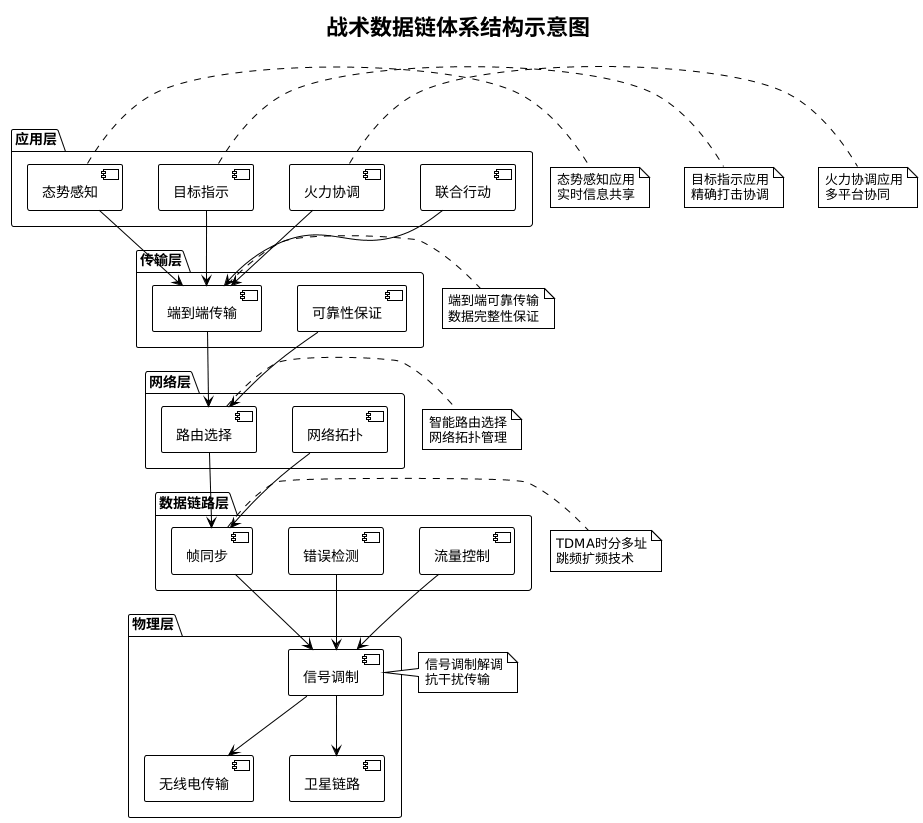
\includegraphics[width=0.8\textwidth,height=0.5\textheight,keepaspectratio]{chapters/fig-0/tdl_architecture_simple.png}
    \caption{战术数据链体系结构示意图}
    \label{fig_tdl_architecture}
\end{figure}

而在北约、美军体系内部,{Link16} 因其具有高速率,抗干扰、加密等特点,被大规模部署到空、海、地等各种平台之中\cite{Ultra_ADSI_2023},被用态势感知、目标标示、火力协同、联合任务等。但随着多链并存、跨域作战等要求的出现,这些原有链路也开始暴露出互操作困难、利用率有限等问题。

Link16的先进性主要体现在其TDMA接入和跳频扩频技术上。TDMA技术是指利用时分多址,多个平台同时工作在同一频段,互不干扰,提高频谱使用效率。Link16跳频扩频技术是指通过快速跳频抗干扰和抗截获,以提高系统的抗干扰性和安全性。Link16采用加密算法对数据进行加密,例如:KGV-8加密机对传输的信息进行加密。

在应用层方面,Link16载荷着各类J系列消息,包括J2.0(基干入网)、J3.0(航迹管理)、J3.2(空中航迹)、J3.3(水面航迹)、J3.5(空中航迹扩展)、J7.0(任务管理)、J12.0(电子战)等。这些消息涵盖着现在作战的方方面面,从简单的航迹消息到复杂的任务协调,为多平台之间的协同作战提供了完整的信息基础。

然而,由于作战的复杂性和作战需求的多样性,Link16也面临着一些挑战。首先是带宽限制问题,虽然 Link16 的传输速率已经较早期系统有很大提高,但是面对大量高清图片、视频等数据的处理能力仍有所欠缺。其次是互操作性问题,不同国家和厂商的设备可能在实现 Link16 标准上存在细微差别,这降低了系统的互操作性。最后是网络安全问题,随着网络攻击手段的不断演进,可能对传统的加密和认证方案形成挑战。

针对这些问题,各个国家国防部队和工业部门均研制有新一代的战术数据链技术,保留Link16优势的前提下,增加带宽、网络安全和与现有技术的兼容性,同时人工智能、机器学习等技术也在一定程度上助力战术数据链技术的智能化进程。

\section{MIL-STD-6016 标准框架与特点}
MIL-STD-6016 作为 {Link16} 的核心标准,对 J 系列报文的格式、语义及应用场景做出了详细规定\cite{ASSIST_6016_2024,CJCSM_6235_01_2025}。其主要特点包括:  

(1)统一的 J 系列消息目录,覆盖作战控制、目标指示与火力支援等功能;  

(2)采用时分多址(TDMA)机制,保证在高密度网络中的有序通信;  

(3)抗干扰能力强,结合跳频扩频和加密算法,提升系统的安全性和鲁棒性;  

(4)具备扩展性,可通过 {JREAP} 协议实现超视距(BLOS)传输,并与 {TTNT} 等新型战术网络互操作。

此外,MIL-STD-6020 明确了跨数据链数据转发与映射的规则;NATO 的 STANAG 5602 及其配套 SIMPLE 规范为异构链路互连提供了标准化接口;而 SISO 标准给出了 {Link16} 仿真的数据模型与交互定义\cite{Ultra_MDLMS_2021}。这些标准共同构成了战术数据链互操作的规范框架。

MIL-STD-6016标准的确立是美军多年来相关战术数据链标准化工作的结果。此标准规定了消息结构、消息语义、J系列消息,并定义了消息处理流程、消息处理错误。每一个消息类型都有明确定义,消息结构、每个字段含义、取值、处理规则等,都为厂商实现设备提供了标准。

图\ref{fig_j_series_message_structure}给出了 MIL-STD-6016 中 J 系列消息的总体框架,展示了消息的分类和组织结构。图中,将 J 系列消息分为六大类:作战控制类(J0-J9)、电子战类(J10-J19)、情报类(J20-J29)和武器协调类(J30-J39),每类消息都有其特定的应用场景和功能定位,体现了标准设计的系统性和完整性。

\begin{figure}[H]
    \centering
    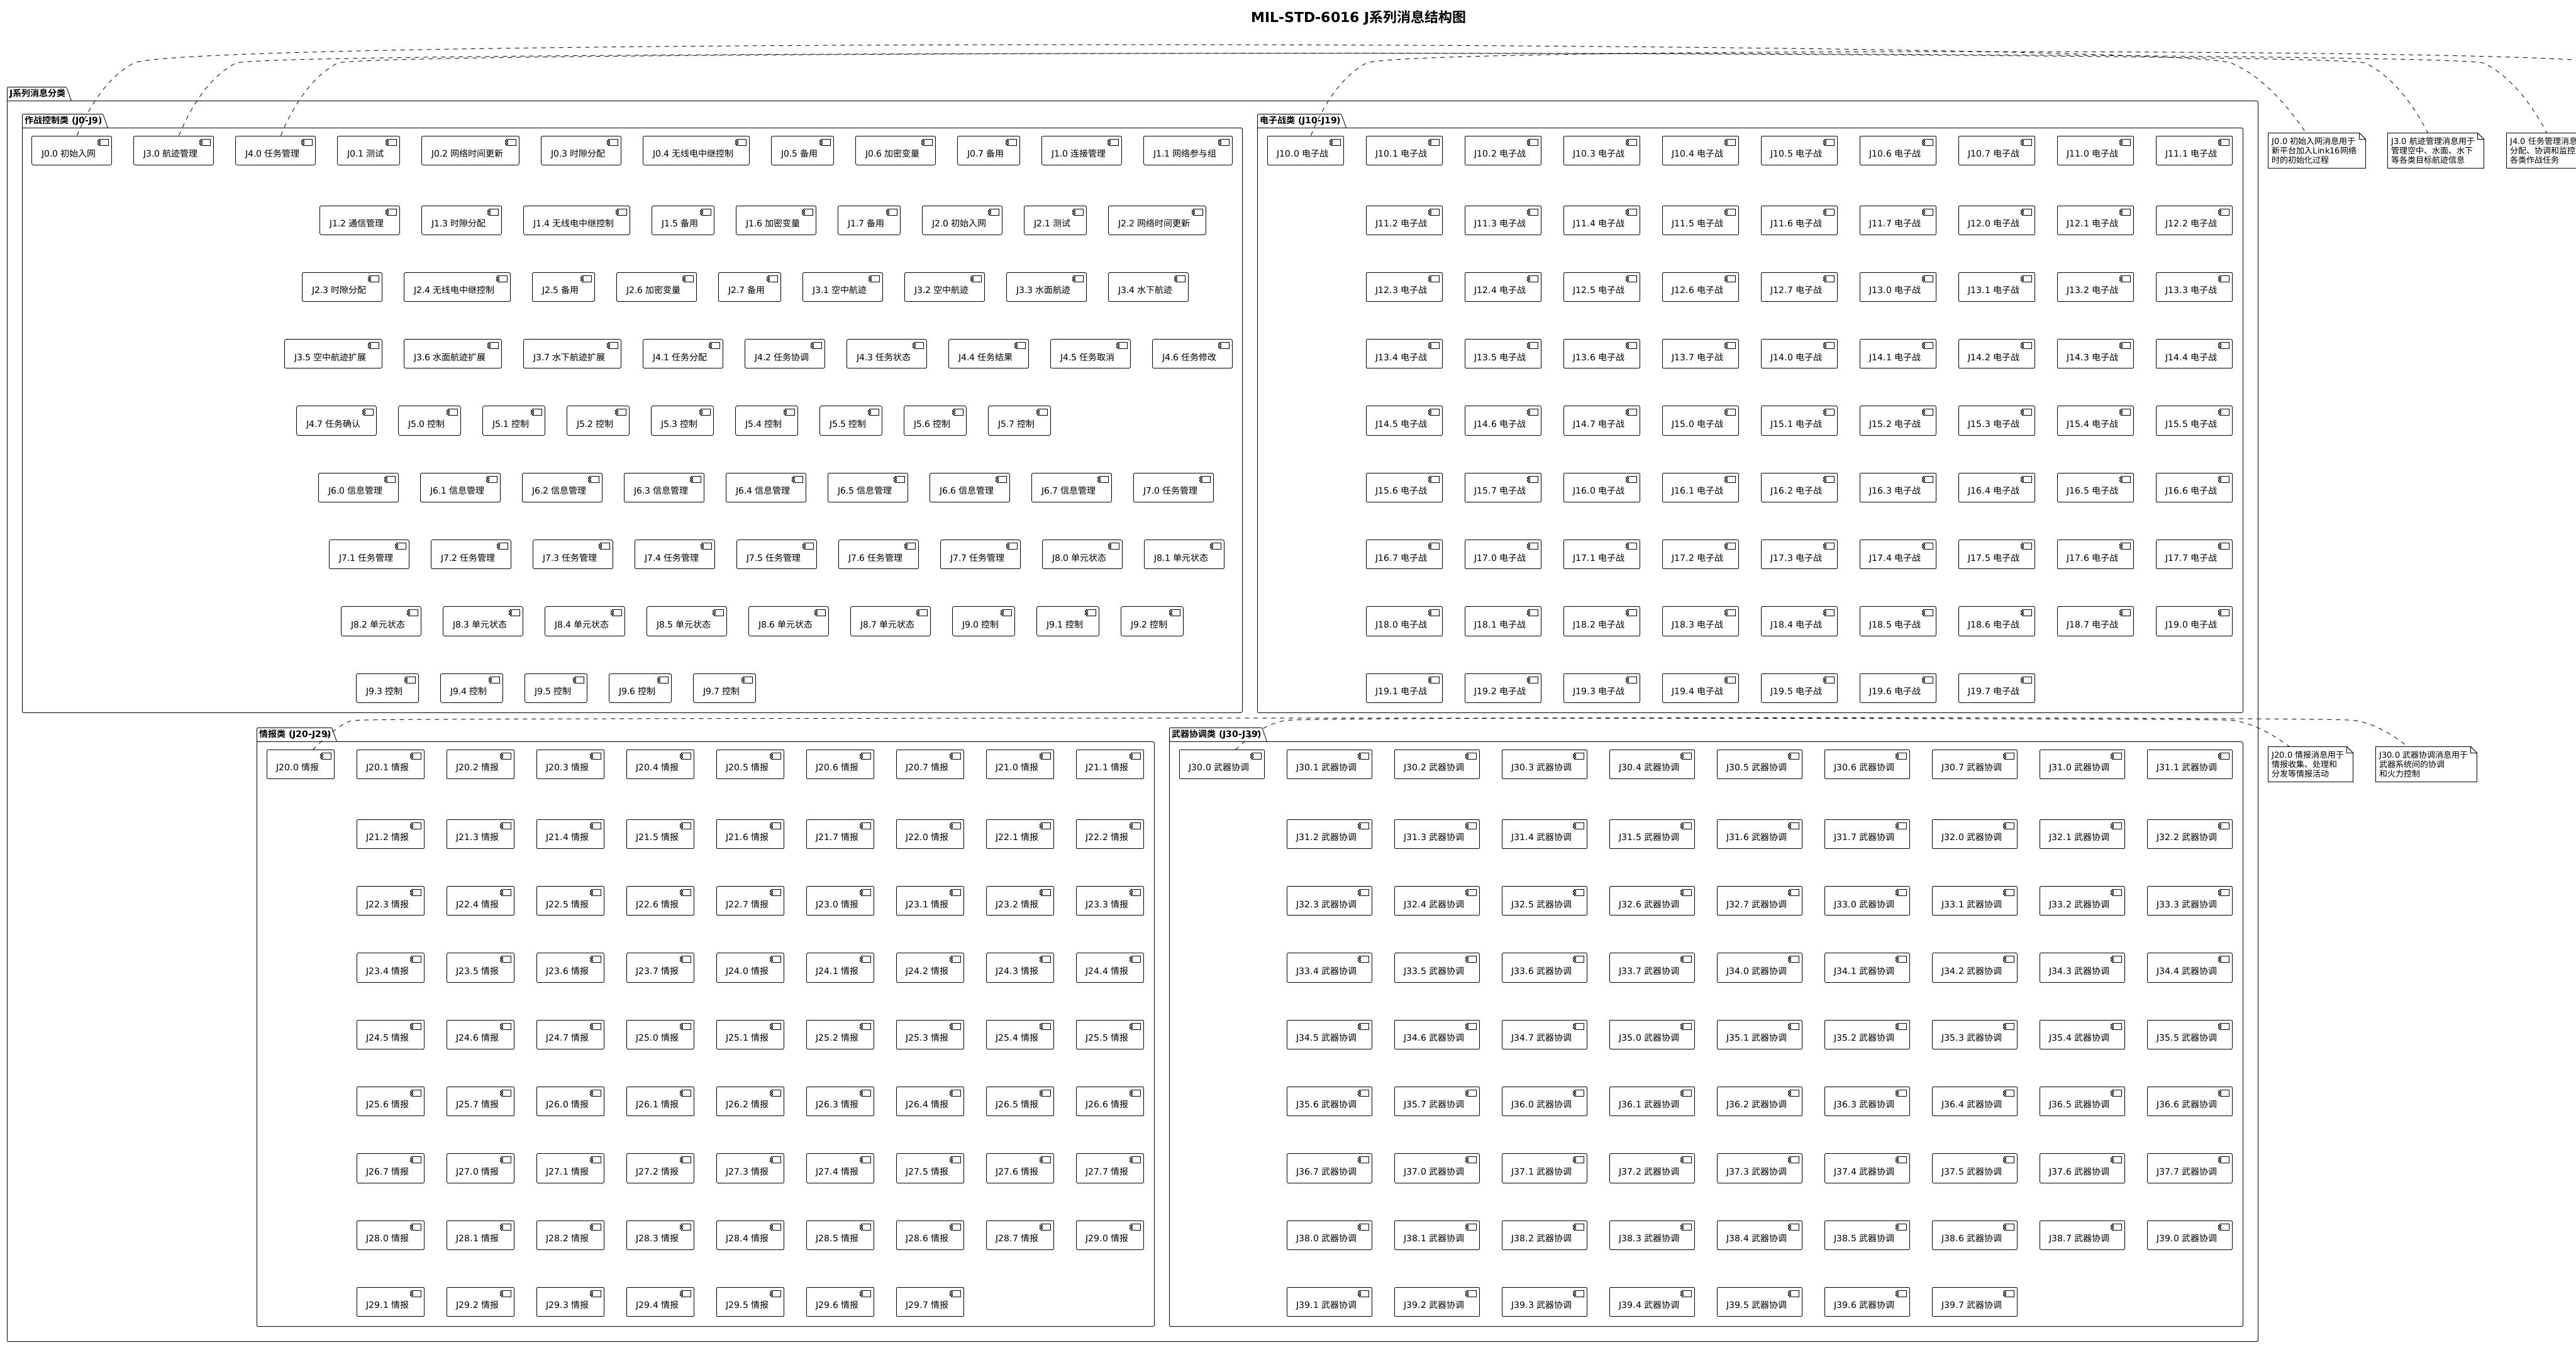
\includegraphics[width=0.85\textwidth,height=0.6\textheight,keepaspectratio]{chapters/fig-0/j_series_message_structure.png}
    \caption{MIL-STD-6016 J系列消息结构图}
    \label{fig_j_series_message_structure}
\end{figure}

在消息格式方面,MIL-STD-6016设计了固定长度消息与可变长度消息,其中固定长度消息处理简单且传输速度快,适合一些实时性要求高的应用,可变长度消息适合于复杂程度不同的消息传输需求,提高了系统的灵活性。这种设计使得Link 16能够同时支持简单的状态报告和复杂的任务协调信息。

标准同时对于消息的语义一致性问题也给予了关注,由于战术数据链涉及到了多军种、多国家平台,消息语义的一致性是互操作能否实现的关键点,在MIL-STD-6016中消息语义一致性的问题通过数据字典、语义规则等的定义使得在不同平台之间信息交互时,对交换信息拥有一致的解析。

随着技术的进步,MIL-STD-6016标准也在不断地发展完善,新版标准在原有基础上扩充了新的消息类型,对原有的一些格式也进行了升级,使其适应新的作战需求和技术发展;此外,增加了网络安全和抗干扰能力,反映了新的作战环境对通信系统安全性的需求。

在标准实施上,美军的各兵种以及工业企业都投入了大量资源来保证标准化的互操作性,包括建立标准化试验、认证、兼容性试验程序来保证MIL-STD-6016在世界范围内的良好实施,为多国联合作战提供技术保障。

表\ref{table_mil_std_comparison}中给出了MIL-STD-6016标准与其他标准的优缺点和应用范围以及互操作能力。在表中可以很清楚的看出MIL-STD-6016标准作为Link16中的核心标准,在消息结构方面、消息传递方面以及互操作性方面都有着独特的优势,是实现战术数据链标准化技术的基础,为战术数据链的互操作提供了一定的技术支持。

\begin{table}[H]
    \caption{MIL-STD-6016相关标准对比分析表}
    \label{table_mil_std_comparison}
    \centering
    \adjustbox{width=0.95\textwidth,center}{%
    \begin{tabular}{lcccc}
        \toprule
        \textbf{标准名称} & \textbf{主要功能} & \textbf{应用范围} & \textbf{互操作性} & \textbf{技术特点} \\
        \midrule
        MIL-STD-6016 & J系列消息格式定义 & Link16战术数据链 & 强 & TDMA、跳频扩频、加密 \\
        & 消息语义规范 & 联合作战平台 & & 固定/可变长度消息 \\
        & 处理流程标准 & 多军种协同 & & 实时性、可靠性 \\
        \midrule
        MIL-STD-6020 & 跨数据链转发 & 多链路互连 & 中等 & 数据映射、格式转换 \\
        & 数据映射规则 & 异构系统集成 & & 协议适配、路由选择 \\
        & 互操作接口 & 联盟作战 & & 标准化接口 \\
        \midrule
        STANAG 5602 & NATO互操作标准 & NATO成员国 & 强 & 统一数据格式 \\
        & SIMPLE规范 & 联盟协同作战 & & 标准化接口 \\
        & 异构链路互连 & 多国联合作战 & & 兼容性保证 \\
        \midrule
        SISO标准 & 仿真数据模型 & Link16仿真系统 & 中等 & 仿真接口标准 \\
        & 交互定义 & 训练与测试 & & 数据模型规范 \\
        & 仿真互操作 & 系统验证 & & 标准化仿真 \\
        \bottomrule
    \end{tabular}%
    }
\end{table}

\section{微服务架构}

微服务架构(Microservice Architecture, MSA)是当今软件工程的最新发展趋势之一,微服务概念的基本思想在2010年前后已经有相关文献提出,James Lewis和Martin Fowler在2014年提出了微服务的概念,是一种以业务能力为中心的模块化架构,具有服务自治、低耦合、可自部署的显著特征,与传统应用程序相比,微服务具有独特的持续交付灵活迅速且可独立模块的能力。2015年,被称为“微服务元年”,Netflix、Amazon、Google等在大规模分布式系统中引入微服务模型,部署服务注册中心、API网关、容错机制,实现服务治理、弹性伸缩、高可用部署,标志着微服务从企业实践逐步走向“学术研究深水区”。

2018-2020年国外学者将研究的重点放在微服务系统的研究及评价上,Waseem\cite{Waseem2021Design}等人基于106份调查问卷和其他调查,对微服务系统的设计、监视和测试做出了总结。他们认为领域驱动的设计(DDD)和基于业务能力服务拆分是目前应用最广泛的设计方式,API网关和Back-end架构是最常用的架构,而资源利用率、负载均衡和日志聚合作为监视的关键领域,微服务工程中模块难以明确、边界划分和自动化测试是普遍存在的问题。此阶段的研究为微服务架构中的质量属性、监视和测试提供了经验,为进一步的研究铺平了道路。

分布式数据系统与云原生技术的发展也为微服务研究注入了新的动力。Laigner等在《Data Management in Microservices》中分析了30多个工业案例和论文,认为Database Per Service模式能够解决跨服务问题和跨服务数据问题,但也会带来数据一致性新问题,需要结合跨服务数据库和Saga模型、事件和最终一致模式来确保可靠性和性能\cite{Laigner2021Data}。后续研究进一步提出面向微服务的基准测试体系,如《Benchmarking Data Management Systems for Microservices》与《Online Marketplace》两篇工作,从事务处理、事件一致性与数据复制角度评估数据管理系统性能,为微服务数据库化演进提供了实验标准 \cite{BenchmarkingDataMgmt2024,OnlineMarketplace2024}。与此同时,Giamattei 等人开展了针对 71 种微服务监控工具的系统性灰文献回顾,总结出资源监控、日志追踪与可观测性平台的实践经验,揭示出当前工具生态存在指标标准不统一与跨层数据整合不足的问题 \cite{MonitoringTools2023}。

安全方面,由于微服务系统的复杂性,也存在基于微服务的访问控制、认证方面的工作。部分工作提出微服务的“零信任”模型,通过轻量级认证(OAuthentication2.0,JWT)和服务网格实现微服务间的安全通信,实现流量分割和细粒度授权。这些工作也进一步促进了未来的 DevSec Operations 和安全问题自动化,国外的学术工作已经关注到了微服务架构的智能和自适应机制设计,通过 AI 和机器学习技术来实现微服务部署调度优化、容器调度、异常发现自动化等,将微服务系统变为动态自适应系统。

国内的微服务研究应用在2010年前后肇始,2007年,阿里巴巴淘宝应用分布式服务框架,开启国内微服务化进程,国内涌现出Dubbo、Spring Cloud阿里巴巴、ServiceComb等一批国产开源框架,企业级系统微服务化应用得到极大发展。2020年前后,国内学者和军工科研机构开始探索复杂信息系统微服务,引入战术通信、指挥控制平台,研究内容主要是服务拆分、容器化、服务编排、跨节点一致控制。一些科研机构开始将微服务集群应用于态势信息处理平台和模拟平台,实现任务模块独立运行和微服务弹性伸缩。国内研究从框架复用和工程应用转向框架设计和性能实验、面向军事通信系统应用的微系统构型开始形成。

图\ref{fig_microservices_evolution_timeline}给出了微服务架构的演进时间轴,从技术理论阶段到智能发展阶段过程清晰,从时间纬度,展示了国外2010年到2014年的概念、理论,2015年到2017年的企业实践、云原生和2018年到2020年的系统研究、2021年至今的智能发展阶段,体现微服务技术的成熟和应用深入。

\begin{figure}[H]
    \centering
    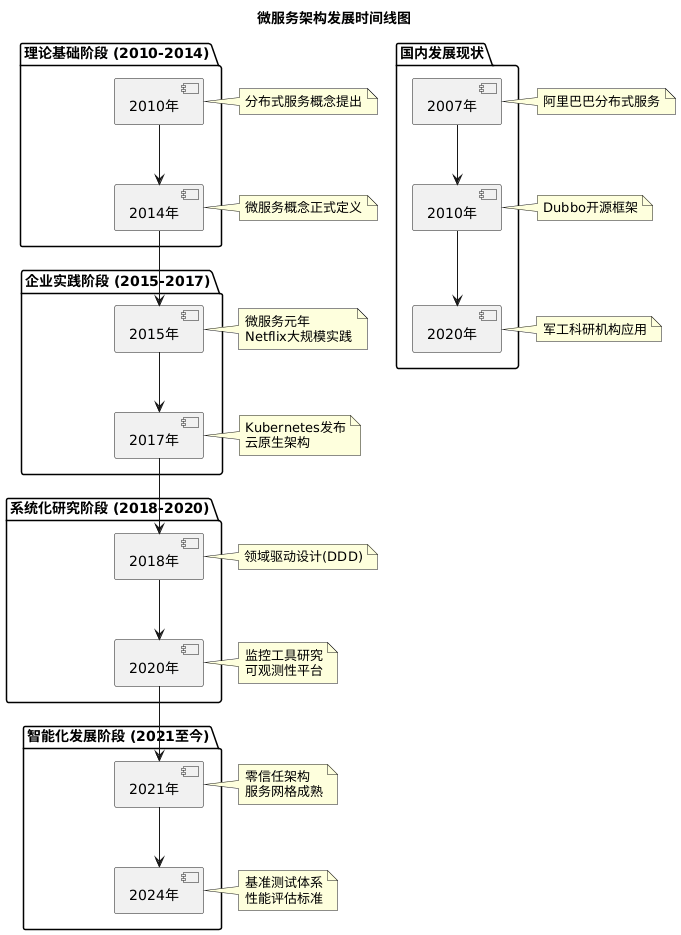
\includegraphics[width=0.8\textwidth,height=0.6\textheight,keepaspectratio]{chapters/fig-0/microservices_evolution_timeline.png}
    \caption{微服务架构发展时间线图}
    \label{fig_microservices_evolution_timeline}
\end{figure}


\section{语义互操作}

语义互操作(Semantic Interoperability)是异构系统在数据交换过程中实现“语义层理解一致”的关键能力,其核心目标是让信息在不同系统、组织或领域间传输时,不仅保持结构一致,还能被准确解释和复用。该概念最早起源于语义网与本体论研究,通过形式化语义模型描述数据背后的概念及其关系,为复杂系统间的理解一致提供理论基础。随着信息系统复杂性与数据异构性的增加,语义互操作逐渐成为人工智能、云计算、医疗健康、工业物联网等领域的核心研究方向。

在国际研究领域,早期的语义互操作工作侧重于标准体系的构建与模型分层。SISO、NATO和ISO等多层互操作模型的提出,将信息互操作划分为语法、语义、语用层\cite{SISO_STD_002_2006,CJCSI_6610_01F_2021},为后续研究提供了一个参考统一体模型。2010年以后,部分学者开始对本体(Ontology)[25]在语义互操作中的应用进行研究。Mishra和Jain提出了“语义知识宝库”(Semantic knowledge treasure),通过OWL和SPARQL完成异构资源统一语义表示和查询\cite{Mishra2018Semantic}。这些研究,标志着语义互操作由概念层面进入知识层面。

近几年,在知识图谱、自动推理、人工智能等技术的推动下,语义互操作研究向智能、自动方向研究。Bernasconi等提出“本体解包”(Ontological Un-packing)方法对已有概念模型进行本体分析,揭示概念模型隐性语义结构,提高模型互操作性\cite{Guizzardi2023Explanation}。Guizzardi 与 Guarino 则在《Semantics, Ontology and Explanation》中引入语义互操作诠释问题,即语义透明性和本体承诺(Ontological Commitment)应作为提高互操作和可理解性和可信赖性的手段\cite{Guizzardi2023Explanation}。此外,机器学习与规则引擎结合的语义映射算法自动获取概念映射关系,进行跨领域知识语义对齐和重用。

随着云与分布式系统应用越来越广泛,语义互操作也扩展到跨平台和多云场景。Hamdan和Admodisastro提出了一种基于本体层(metalayer)的多云语义互操作参考模型,并在参考模型基础上设计了语义中心(Semantic Hub)用来协调不同云场景中的语义模型,并提供语义一致性服务\cite{Hamdan2023Reference,SemanticMultiCloud2024}。同时指出,在异构场景中保持语义一致性需要在三个模型层进行协同,即架构层、数据层和治理层;同时语义互操作也在与数据治理、知识发现、可解释人工智能等研究进行深度融合,为跨平台和协同提供基础能力。

国内语义互操作研究源于 2000 年代的语义网工程,近年来知识图谱和人工智能的兴起,进一步推动了语义互操作研究。语义本体构建、语义映射方法、语义信息检索、语义推理机制等研究热度持续攀升。以知识图谱为研究对象,在构建语义关系模型的基础上,对异构数据进行实体映射、语义标注,从而实现可融合性;以智慧城市、医疗、交通、工业互联网应用为研究对象,以语义互操作为核心,研究多源数据融合与协同管理。语义互操作研究从“语义建模”转向“语义计算”的研究,以语义理解、语义推理和动态本体演化为核心,满足即时性、可解释性强的新需求。

语义互操作体系结构层次从物理层到语用层共分为4层架构模式。具体语义互操作系统体系结构的层次如\ref{fig_semantic_interop_architecture}所示,物理层实现传输协议和网络互联,语法层实现数据格式、消息结构,语义层实现本体模型和概念映射,语用层实现业务规则、上下文理解等,互操作机制中的语义中枢、映射引擎、转换器、验证器体现了语义互操作技术的抽象和完整性。

\begin{figure}[H]
    \centering
    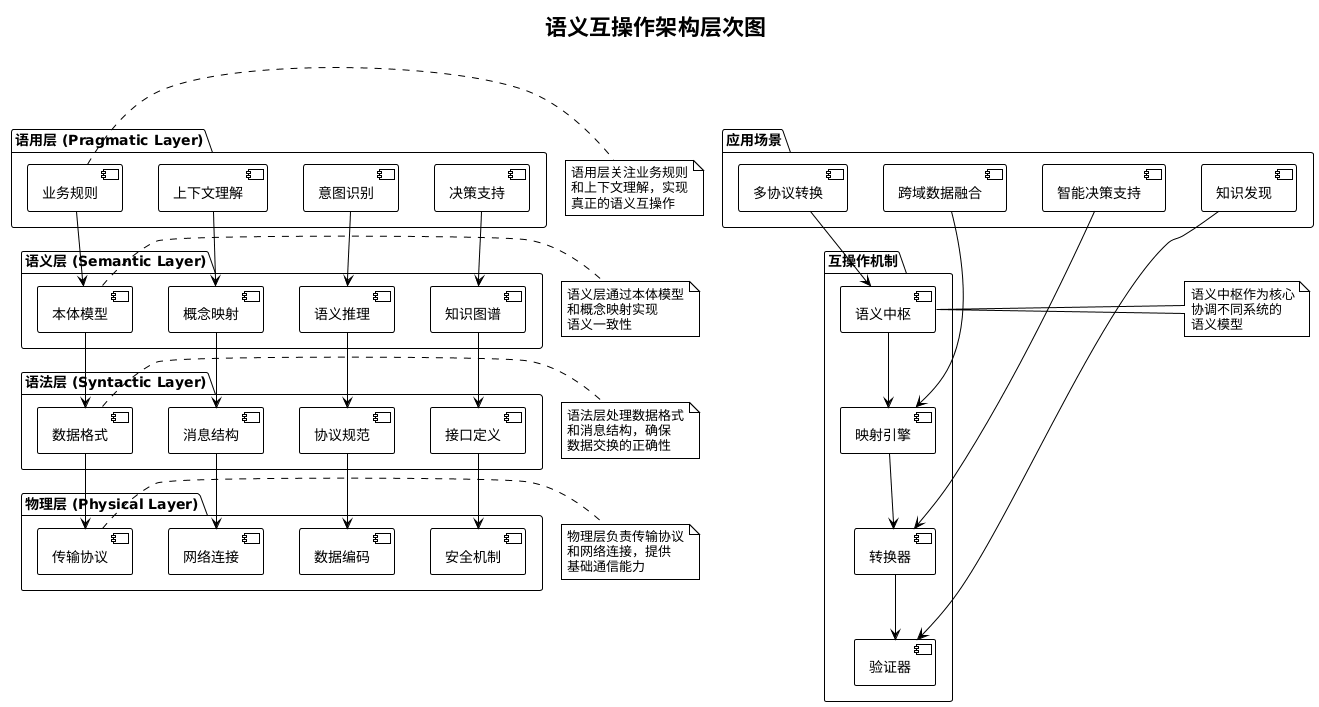
\includegraphics[width=0.85\textwidth,height=0.7\textheight,keepaspectratio]{chapters/fig-0/semantic_interop_architecture.png}
    \caption{语义互操作架构层次图}
    \label{fig_semantic_interop_architecture}
\end{figure}


\section{自动化处理}

自动化处理技术是复杂信息系统中的必要技术,主要是为了将非结构化(半结构化)文档(PDF、Word、XML、JSON等文件)进行自动解析、识别、导入数据库或其他知识系统中进行高效、精准的建模和信息抽取,经过了基于规则的处理到机器学习、深度学习等智能处理的发展历程,近年来,在自然语言处理、智能文档处理(Document Intelligence)、多模态学习等方面取得了快速发展。

早期的自动化文档处理研究以版面分析(Layout Analysis)和文本块识别为主要方法。典型工作包括基于光学字符识别(OCR)的文本抽取、表格检测与区域定位算法。这一阶段的研究主要依赖启发式规则与图像分割算法,如 PDFMiner、Apache Tika 等工具框架,通过对文本流与版面结构的分析实现基本的内容解析。然而,这些方法难以处理复杂文档中的语义结构与跨页逻辑关系。

随着深度学习和自然语言识别的发展,更多基于网络的文档识别和语义理解模型被提出。2020年起,Google、Microsoft、Adobe等机构使用视觉语言联合模型(Vision-language Models)进行文档识别和文档阅读任务\cite{Xu2020LayoutLM,Xu2022LayoutLMv3},Xu等使用联合模型对文本、位置和视觉信息进行建模,对文档结构和语义进行理解和识别,如表单识别、关键字识别、文档分类等。论文中的基于Tensor多模态的方法在识别PDF结构时获得了不错的效果。该方法为复杂结构文档识别提供了一个通用的框架。

在信息抽取与结构化导入方向,学者们提出了多种智能抽取与标准映射框架。Li 等在《DocParser: Document Parsing and Structured Data Import》\cite{Li2021DocParser} 中提出一种结合文本分块、实体识别与模板匹配的自动导入机制,实现 PDF 与 XML 文档的语义级结构化导入。与此同时,研究者将知识图谱构建与自动文档处理相结合,通过实体识别、关系抽取与语义对齐实现从原始文档到知识图谱的自动生成,为数据标准化与语义互操作奠定了基础。此类方法已在专利文档、医学报告与技术标准文件的自动建模中得到验证。

近年来,自动化加工逐渐发展到自动化的监督学习和跨模态理解,模型不再需要人工标注而是采用海量的通用特征预训练而成,例如Powalski等人提出的文档自动分类与提取表格任务中的文本-视觉双流Transformer模型\cite{Powalski2021DocFormer}。随后,将大规模语言模型(LLM)与文档知识关联起来的跨模态语义推理与任务自适应成为研究热点\cite{Wang2023DocumentLLM},文档自动化迎来了“语义理解为王”的新时代。

国内对于自动化文档处理的研究集中于结构化识别和智能导入系统的工程化运用,研究院所及科技企业进行了对于PDF解析、表格抽取、标注字段、标准导入的研究,开发基于深度学习的OCR引擎、语义分层引擎,百度文心、阿里达摩院、华为诺亚方舟实验室等都提出了面向企业文档及技术标准的多种模态解析思路,并部分运用到企业电子政务、科研档案、装备资料中。然而,国内研究仍具有跨格式迁移能力差、语义抽象层次低、自动验证及纠错能力不足的问题,在知识表示、语义约束及可解释性方面需进一步加强。

图\ref{fig_document_processing_evolution}描述了文档的自动处理技术演化轨迹,描绘了规则驱动、机器学习、深度学习等4个阶段。从技术维度勾勒了文档自动处理技术的4个发展演进轨迹,从2000-2010年的启发式算法的规则驱动阶段,到2010-2020年的视觉语言融合模型阶段,再到2020-2023年的深度学习的Tensor架构阶段,以及2023年以来的文档自动处理技术智能化阶段,涉及电子政务、科研档案、装备资料、技术标准等各个领域。

\begin{figure}[H]
    \centering
    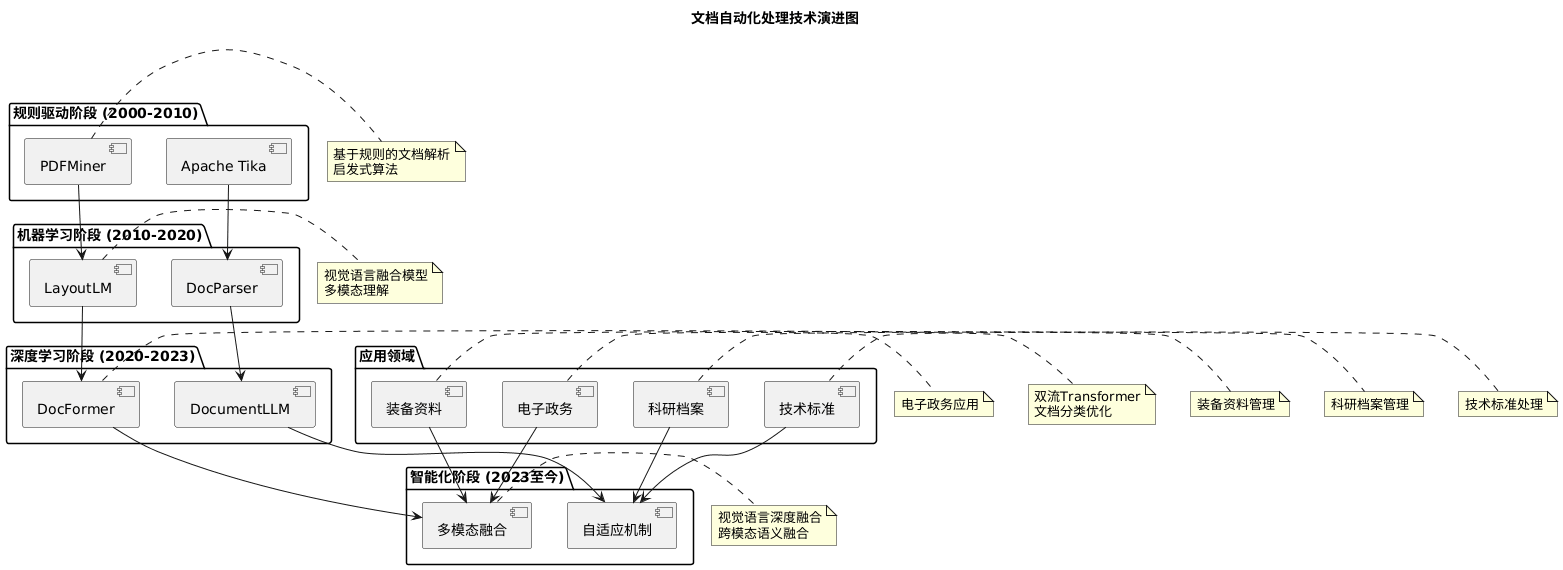
\includegraphics[width=0.8\textwidth,height=0.6\textheight,keepaspectratio]{chapters/fig-0/document_processing_evolution.png}
    \caption{文档自动化处理技术演进图}
    \label{fig_document_processing_evolution}
\end{figure}

\section{本章小结}

基于以上分析,本章系统梳理了战术数据链技术、微服务架构和语义互操作三个核心技术领域的理论基础、发展现状和技术特点。通过深入分析相关技术的研究进展和应用实践,为构建基于MIL-STD-6016标准的战术数据链信息标准数据库系统提供了坚实的理论基础。

在战术数据链技术方面,MIL-STD-6016标准为J系列消息的格式化和语义化提供了统一规范,为系统设计提供了标准依据。在微服务架构方面,其分布式、模块化的设计理念为构建高性能、高可用的数据库系统提供了技术支撑。在语义互操作方面,基于本体的语义映射机制为实现跨标准的数据融合和互操作提供了关键技术路径。

基于以上技术分析,本研究将采用微服务架构构建战术数据链信息标准数据库系统,通过语义互操作技术实现MIL-STD-6016消息的标准化存储、语义化处理和跨标准互操作,为多链融合提供统一的信息支撑平台。下一章将详细阐述系统的总体架构设计和核心算法研究。

